% This example is meant to be compiled with lualatex or xelatex
% The theme itself also supports pdflatex
\PassOptionsToPackage{unicode}{hyperref}
\documentclass[aspectratio=1610, 9pt]{beamer}

% Load packages you need here
\usepackage{polyglossia}
\setmainlanguage{german}
\setmonofont{Libertinus Mono}
\usepackage{csquotes}
    

\usepackage{amsmath}
\usepackage{amssymb}
\usepackage{mathtools}

\usepackage{hyperref}
\usepackage{bookmark}
\usepackage{color}


% load the theme after all packages

\usetheme[
  showtotalframes, % show total number of frames in the footline
]{tudo}

% Put settings here, like
\unimathsetup{
  math-style=ISO,
  bold-style=ISO,
  nabla=upright,
  partial=upright,
  mathrm=sym,
}

\title{Strukturfunktionen}
\author[L.~Kolk]{Lars Kolk}
\institute[Fakultät Physik]{Fakultät Physik}
%\titlegraphic{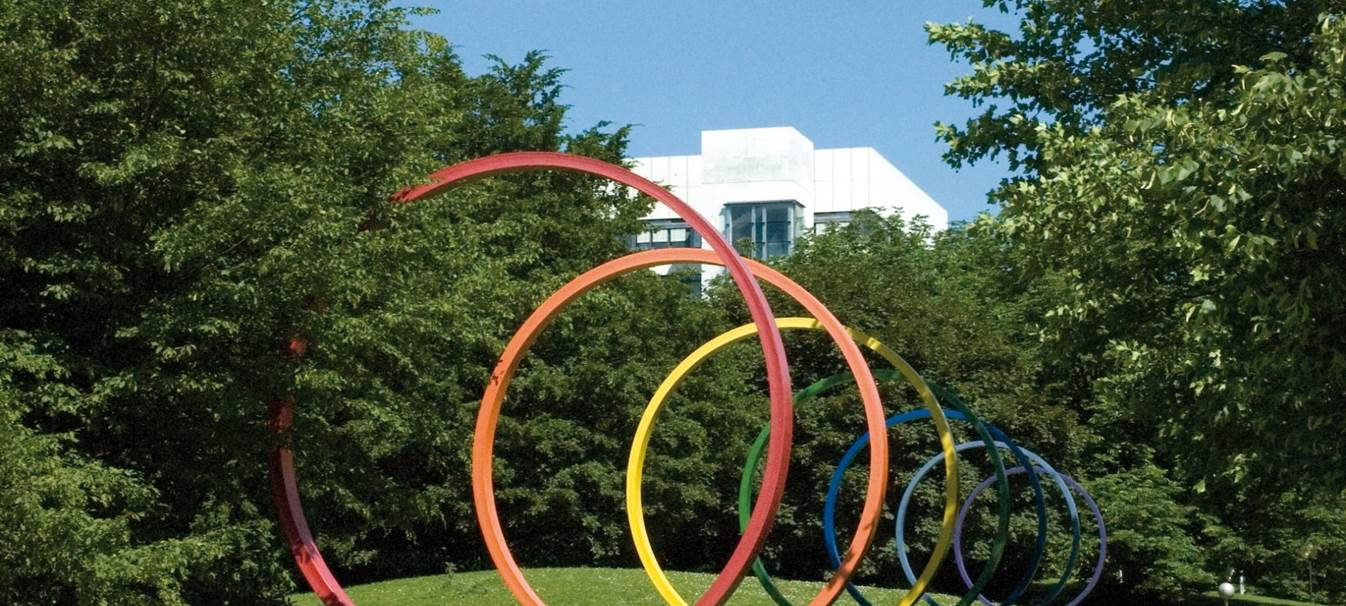
\includegraphics[width=0.7\textwidth]{images/tudo-title-2.jpg}}


\begin{document}

\maketitle


\begin{frame}{Einführung}
  \tableofcontents
\end{frame}

\section{Motivation}
\subsection{Das Proton}
\begin{frame}{Das Proton}
\begin{columns}
\begin{column}{0.40\textwidth}
  \includegraphics[width = \textwidth]{images/atom.png}
\end{column}
\begin{column}{0.60\textwidth}
    Protonen:
    \begin{itemize}
      \item{bilden zusammen mit Neutronen den Atomkern}
      \item{sind Baryonen}
      \item{haben eine einfach positive Ladung}
      \item{haben eine Masse von $938,272081 \pm 0,000006 \,\mathrm{MeV}$ }
      \item{besteht aus zwei Up- und einem Downquark (Valenzquarks)}
    \end{itemize}
\end{column}
\end{columns}
\end{frame}

\begin{frame}{Die Valenzquarks}
  \begin{columns}
    \begin{column}{0.40\textwidth}
      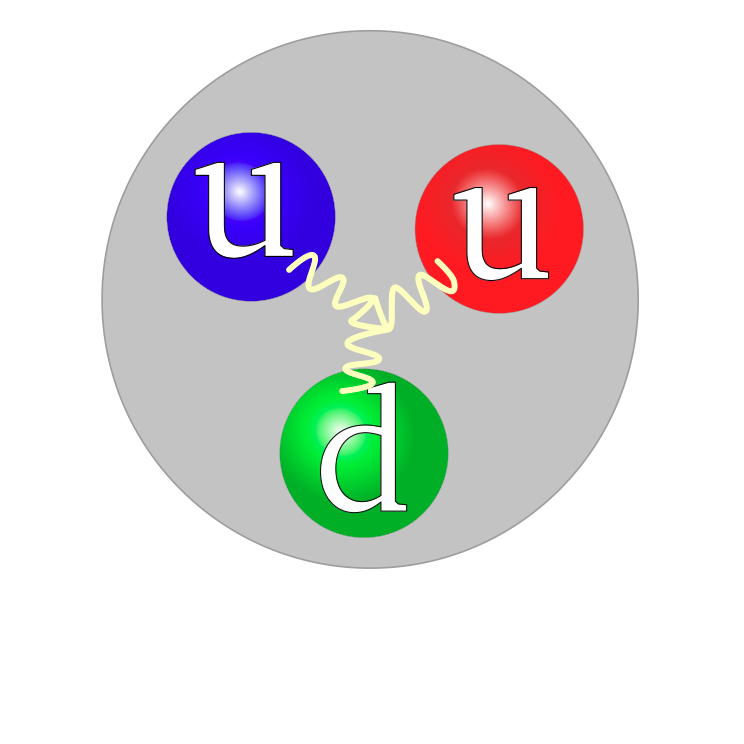
\includegraphics[width = \textwidth]{images/Proton.png} 
    \end{column}

    \begin{column}{0.45\textwidth}
      Das Up-Quark:
      \begin{itemize}
        \item{ $ m_\text{u} = 2,16 \substack{+0.49 \\ -0.26} \,\mathrm{MeV} $  }
        \item{ $ q_\text{u} = \frac{2}{3} e$ }
      \end{itemize}
      
      Das Down-Quark:
      \begin{itemize}
        \item{ $ m_\text{d} = 4,67 \substack{+0.48 \\ -0.17} \,\mathrm{MeV} $  }
        \item{ $q_\text{d} = - \frac{1}{3} e$ }
      \end{itemize}

      Gesamt:
      \begin{itemize}
        \item{ $ m_\text{ges} = 8,99 \substack{+1,09 \\ -0.55} \,\mathrm{MeV} $  }
        \item{ $ q_\text{ges} =  e$ }
      \end{itemize}      

    \end{column}
  \end{columns}
\end{frame}

\subsection{Das Rutherford Experiment}
\begin{frame}{Rückblick: Das Rutherford Experiment}
  \begin{columns}
    \begin{column}{0.4\textwidth}
      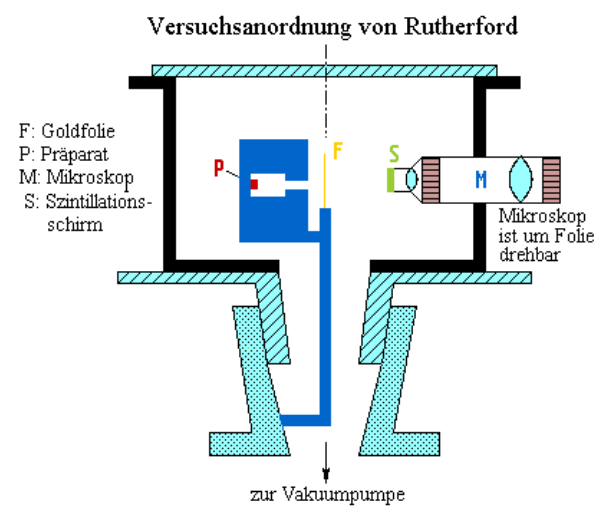
\includegraphics[width=\textwidth]{images/Rutherford1.png}
    \end{column}
    \begin{column}{0.6\textwidth}
      \begin{itemize}
      \item{Streuung von $\alpha$-Teilchen an Goldfolie}
      \item{Durchgeführt: }
      \begin{itemize}
        \item{1908-1913}
        \item{von Hans Geiger und Ernest Marsden unter Führung von Ernest Rutherford}
      \end{itemize}
      \item{Beobachtung: }
      \begin{itemize}
        \item{Ein Großteil der $\alpha$-Teilchen fliegt durch die Folie hindurch}
        \item{Bei einigen wenigen $\alpha$-Teilchen kam es zu einer Streuung}
      \end{itemize}
      \item{Folgerung:}
      \begin{itemize}
        \item{Das Thomsonsche Atommodell ist nicht vollständig}
        \item{Masse des Atoms muss in einem Kern konzentriert sein}
        \item{Atom größenteils leer}
      \end{itemize}
      \end{itemize}
    \end{column}
  \end{columns}
\end{frame}

\begin{frame}{Rutherford-Streuformel}
  \begin{columns}
    \begin{column}{0.4\textwidth}
      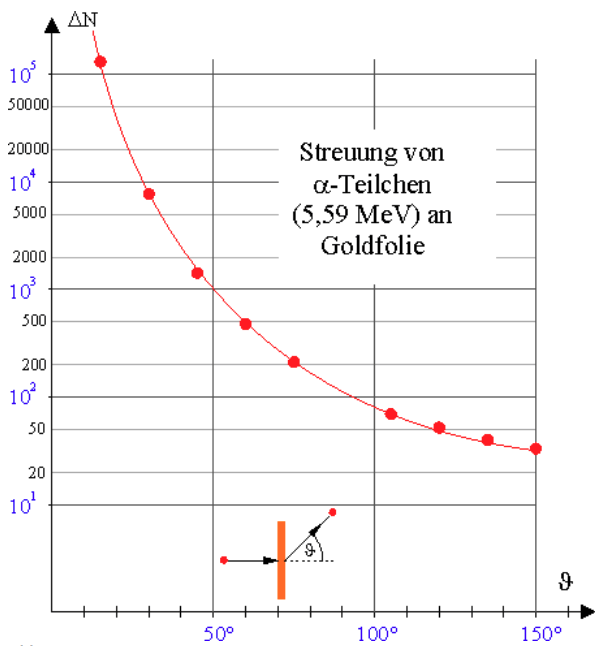
\includegraphics[width=\textwidth]{images/Streuung.png}
    \end{column}
    \begin{column}{0.6\textwidth}
      \begin{itemize}
        \item{Plot zeigt wie viele Teilchen $\Delta D$ pro Streuwinkel $\vartheta$ auftreten}
        \item{Es lässt sich die Rutherford-Streuformel finden:}
        \begin{itemize}
        \item{$ \frac{\symup{d} \sigma}{\symup{d} \Omega } = \left( \frac{Z_\text{1}Z_\text{2} e^2}{16 \pi \epsilon_\text{0} E_\text{kin}} \right)^2 \cdot \frac{1}{\sin^4{\frac{\vartheta}{2}}} $}
        \item{$Z_\text{1} \,\hat{=}  \,\text{Anzahl der Ladungsträgern des gestreuten Teilchen} $, $Z_\text{2} \,\hat{=}  \,\text{Ordnungszahl des Targets} $}  
        \end{itemize}
      \end{itemize}
    \end{column}
  \end{columns}
\end{frame}

\subsection{Elektronstreuung}
\begin{frame}{Elektronstreuung}
  \begin{columns}
    \begin{column}{0.6\textwidth}
  Betrachtung von Elektronstreuung
      \begin{itemize}
        \item{ab den 1950ern können Elektronen leicht erzeugt und beschleunigt werden}
        \item{$E_\text{kin} = 100 \,\mathrm{MeV} \rightarrow \lambda = 12\,\mathrm{fm} $}
        \item{Einfluss von Spin-Bahn-Kopplung $\rightarrow$ Modifikation der Rutherford-Streuformel}
      \begin{itemize}
         \item{$ \left( \frac{\symup{d} \sigma}{\symup{d} \Omega } \right)_\text{Mott} = \left( \frac{\symup{d} \sigma}{\symup{d} \Omega } \right)_\text{Ruth} \cdot \left( 1-\frac{v^2}{c^2} \sin^2{ \frac{\vartheta}{2} } \right) $}
      \end{itemize} 
      \end{itemize}
    \end{column}

  \begin{column}{0.4\textwidth}
    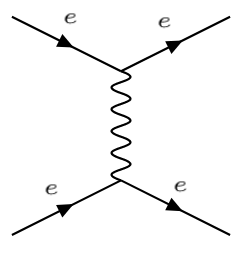
\includegraphics[scale=0.3]{images/ee-scattering.png}
  \end{column}

  \end{columns}
\end{frame}

\subsection{Ladungsverteilung und Formfaktoren}
\begin{frame}{Ladungsverteilung und Formfaktoren}
\begin{itemize}
  \item{Bisher: Punktförmige Ladung}
  \item{Nun: Ladungsverteilung $\rightarrow$  (erneute) Modifikation des Wirkungsquerschnittes}
  \begin{itemize}
    \item{$\left( \frac{\symup{d} \sigma}{\symup{d} \Omega } \right) = \left( \frac{\symup{d} \sigma}{\symup{d} \Omega } \right)_\text{Mott} \cdot \left| F(\vec{q}) \right|^2 $}
    \item{$F(\vec{q}) = \displaystyle \int{ exp{\left(\frac{i}{\hbar} \vec{x} \vec{q} \right)} \rho(\vec{x}) \symup{d}\vec{x} } $}
    \item{$\vec{q} \,\hat{=} \,\text{Impulsbeitrag} $, $\rho \,\hat{=} \,\text{Ladungsverteilung} $}
  \end{itemize}
\end{itemize}

\end{frame}


\begin{frame}
\centering
  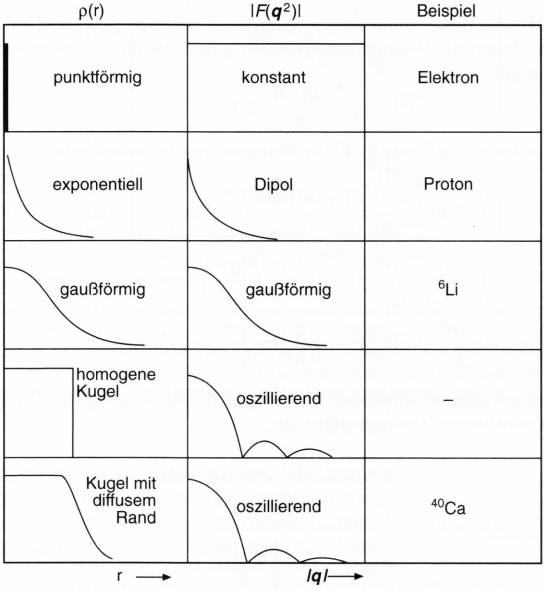
\includegraphics[scale=0.35]{images/Form.png}
\end{frame}

\begin{frame}
\centering
  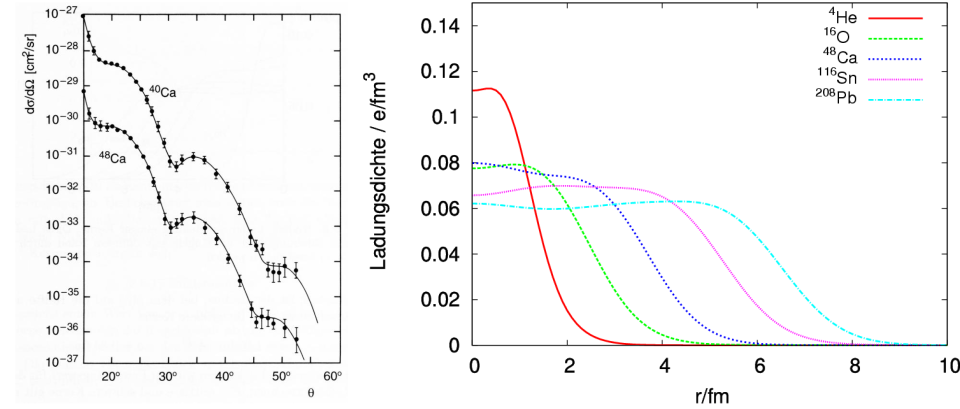
\includegraphics[scale=0.4]{images/Ladungsverteilung.png}
\end{frame}

\begin{frame}{Warum ist das wichtig?}
  \begin{itemize}
    \item{Bereits kleine Energien liefern Aussage über Ladungsverteilung}
    \item{Können bei größeren Energien Aussagen über die Struktur von Proton getroffen werden?}
    \begin{itemize}
      \item{Kurze Antwort: Ja!}
    \end{itemize}
  \end{itemize}
\end{frame}

\section{Struktur des Protons}


\begin{frame}{Struktur des Protons}
  \begin{itemize}
    \item{Bisher:}
    \begin{itemize}
      \item{Energien im $\mathrm{MeV}$-Bereich }
      \item{Elastische Streuung}
      \item{Aussage über Ladungsverteilung}
    \end{itemize}
    \item{Nun:}
    \begin{itemize}
      \item{Energien im $\mathrm{GeV}$-Bereich}
      \item{(Tief-)inelastische Streuung}
      \item{Aussage über die Struktur des Protons}
    \end{itemize}
  \end{itemize}
\end{frame}

\subsection{Inelastische Streuung}
\begin{frame}{Inelastische Streuung}
  Beispiel:
  \begin{figure}[H]
  \centering
  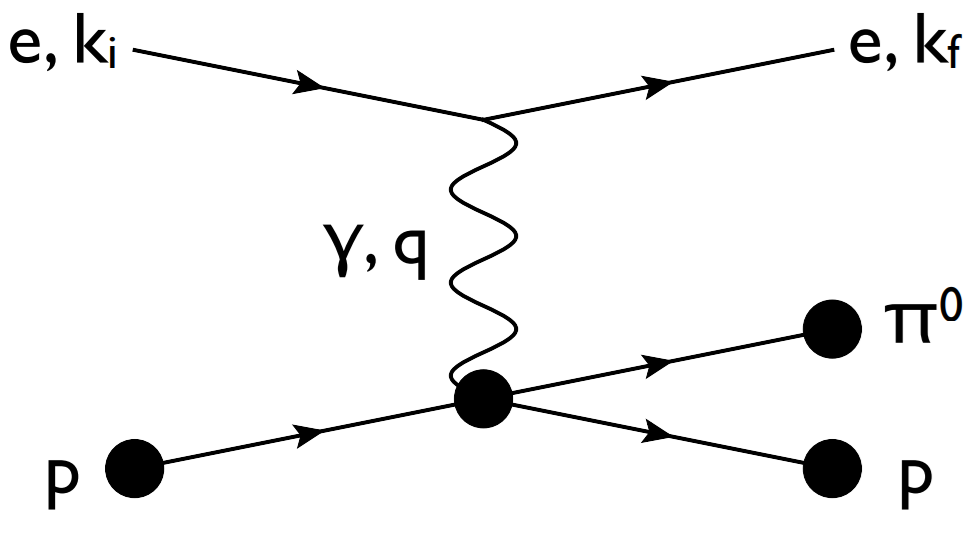
\includegraphics[width=0.7\textwidth]{images/inelastic.png}  
  \end{figure}
  Gut, aber noch keine Information über Quark-Struktur
\end{frame}

\subsection{Tief-inelastische Streuung}
\begin{frame}{Tief-inelastische Streuung}
\begin{figure}
  \centering
  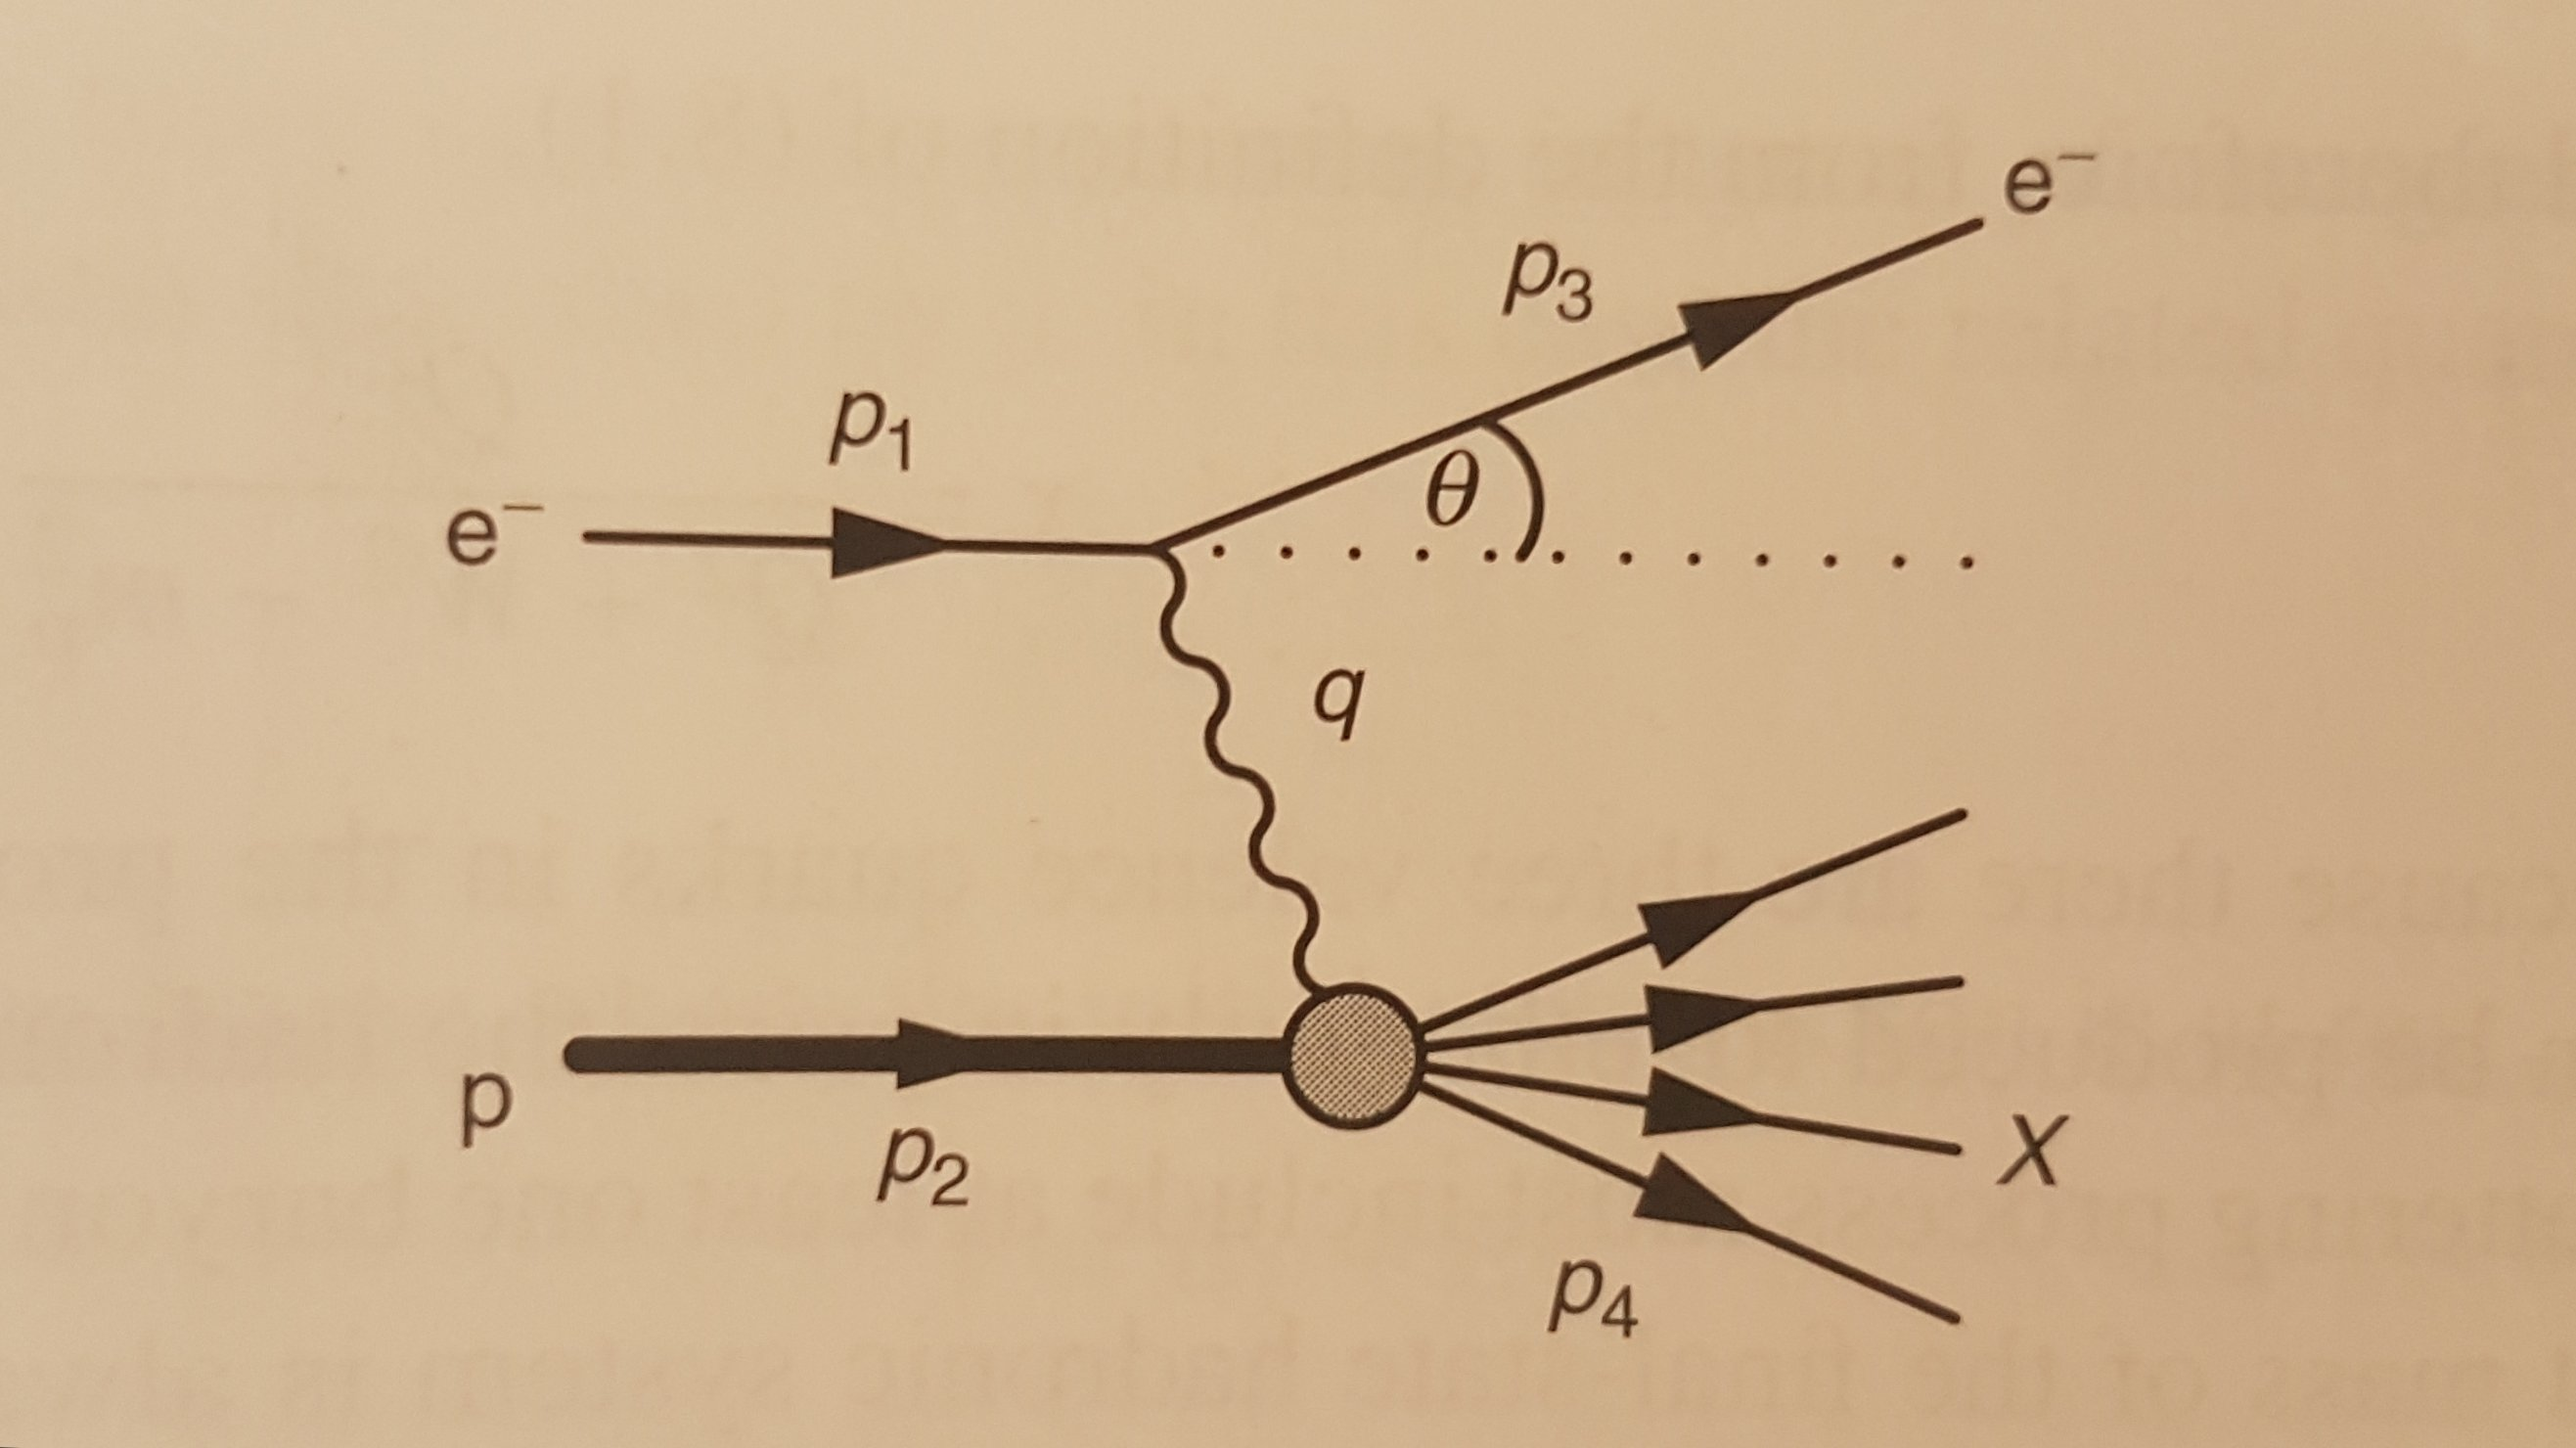
\includegraphics[width=0.7\textwidth]{images/ep-deep-inelastic-scattering-1.jpg}
\end{figure}
\end{frame}

\begin{frame}{Wirkungsquerschnitt}
\begin{itemize}
  \item{Ansatz über Rosenbluth, da:}
  \begin{itemize}
    \item{relativistisch gerechnet werden muss}
    \item{Vierervektoren statt Vektoren}
  \end{itemize}
  \item{Rosenbluth:}
  \begin{itemize}
    \item{ $ \frac{\symup{d} \sigma}{\symup{d} \Omega }  = \frac{\alpha^2}{4 E^2_1 sin^4{\frac{\vartheta}{2}}} \cdot \frac{E_3}{E_1} \left( \frac{G^2_\text{E}+ \tau G^2_\text{M}}{1+\tau} cos^2{\frac{\vartheta}{2}} +2\tau G^2_\text{M} sin^2{\frac{\vartheta}{2}} \right) $}
    \item{ $ \tau = \frac{Q^2}{4m_\text{p}} $ }
    \item{ $ Q^2 = -(p_1-p_3)^2$ }
    \item{ $y = 1-\frac{E_3}{E_1} $ }
    \item{$G_\text{i} \,\hat{=} \, \text{Formfaktoren, die die Verteilung der Ladung und des magnetischen Moments beschreiben}$}
  \end{itemize}
\end{itemize}  
\end{frame}

\begin{frame}
  \begin{itemize}
  \item{Rosenbluth kann umgeschrieben und verallgemeinert werden zu: }
  \begin{itemize}
    \item{$ \frac{\symup{d}^2\sigma}{ \symup{d}x \symup{d}Q^2} = \frac{4 \pi \alpha^2}{Q^4} \left[ \left( 1 - y - \frac{m^2_\text{p} y^2}{Q^2} \right) \frac{F_2(x, Q^2)}{x} + \frac{1}{2}y^2F_1(x, Q^2) \right]  $}
    \item{$F_\text{i} \,\hat{=} \, \text{Formfaktoren} $}
    \begin{itemize}
      \item{$F_1 \,\hat{=} \, \text{Magnetischer Formfaktor} $}
      \item{$\text{Spin} = 0 \rightarrow F_1 = 0$}
    \end{itemize}
    \item{$x \,\hat{=} \text{Bjorken x} \equiv \frac{Q^2}{2 p_2 q} $}
    \item{tief-inelastische Streuung $\rightarrow Q^2 \gg  m^2_\text{p} y^2 $}
  \end{itemize}
  \end{itemize}
\end{frame}

\begin{frame}{Bjorken-Scaling}
  \begin{columns}
    \begin{column}{0.4\textwidth}
      \begin{itemize}
        \item{Erste Studien am Stanford Linear Accelerator Center (SLAC) in Californien}
        \item{Untersucht:}
        \begin{itemize}
          \item {inelastische Elektron-Proton-Streuung}
          \item {$E_\text{e} = (5 - 20) \,\mathrm{GeV} $}
          \item {Elektronen wurden auf flüssiges Wasserstoff-Target geschossen}
        \end{itemize}
        \item{Beobachtung:}
        \begin{itemize}
          \item {$F_1(x, Q^2)$ und $F_2(x, Q^2)$ sind unabhängig von $Q^2$}
          \item {Callan-Gross-Beziehung: $F_1(x, Q^2) = 2 F_2 x (x, Q^2)$}
        \end{itemize}
        \item{Folgerung:}
        \begin{itemize}
          \item {Das Proton besteht aus punktförmigen Spin $\frac{1}{2}-Teilchen $ }
        \end{itemize}
      \end{itemize}
    \end{column}
    \begin{column}{0.6\textwidth}
      \begin{figure}
        \centering
        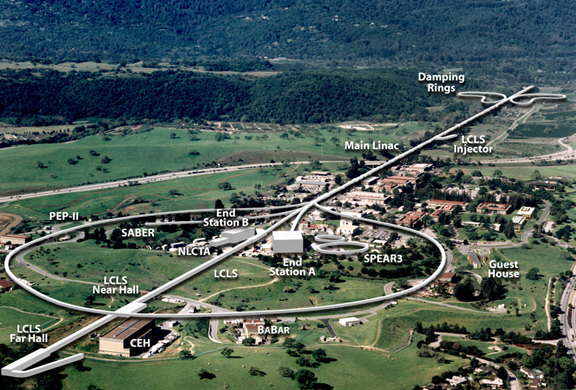
\includegraphics[width=0.75\textwidth]{images/ariel2.jpg}
      \end{figure}
    \end{column}
  \end{columns}
    
\end{frame}

\subsection{Proton-PDF}

\begin{frame}{Proton-PDF}
\begin{columns}
  \begin{column}{0.45\textwidth}
    \begin{figure}
    \centering
    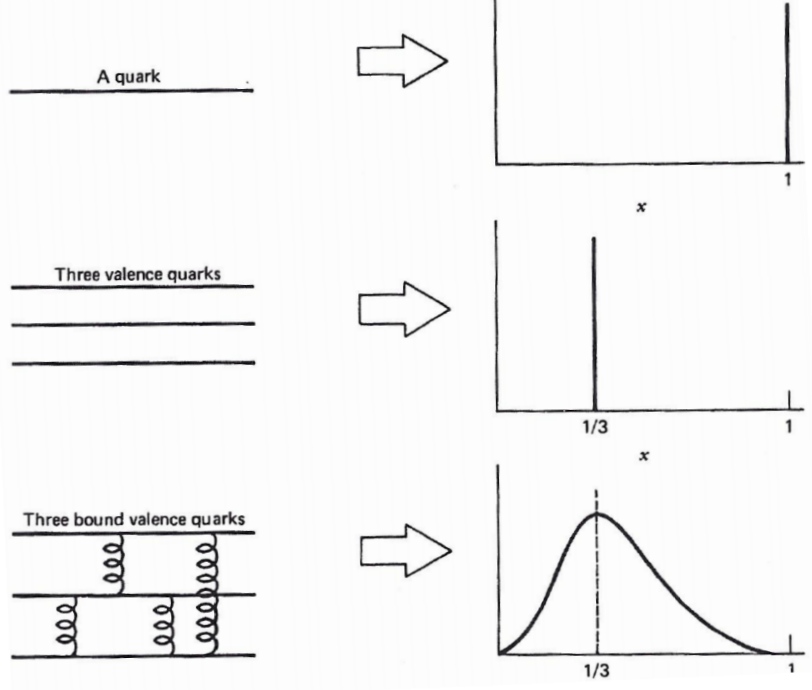
\includegraphics[width=0.8\textwidth]{images/Bjorken-1.png}
  \end{figure}
  \begin{figure}
    \centering
    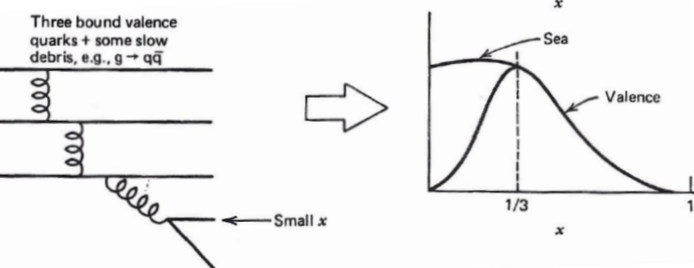
\includegraphics[width=0.8\textwidth]{images/Bjorken-2.png}
  \end{figure}
  \end{column}
  \begin{column}{0.55\textwidth}
    \begin{itemize}
      \item{Bjorken-x entspricht Impulsbruchteil eines Partons}
      \item{Betrachtung der Parton-Verteilungsfunktion}
    \end{itemize}
  \end{column}
\end{columns}
\end{frame}


\section{Hera am DESY}

\begin{frame}{Hera am DESY}
  \begin{figure}
    \centering
    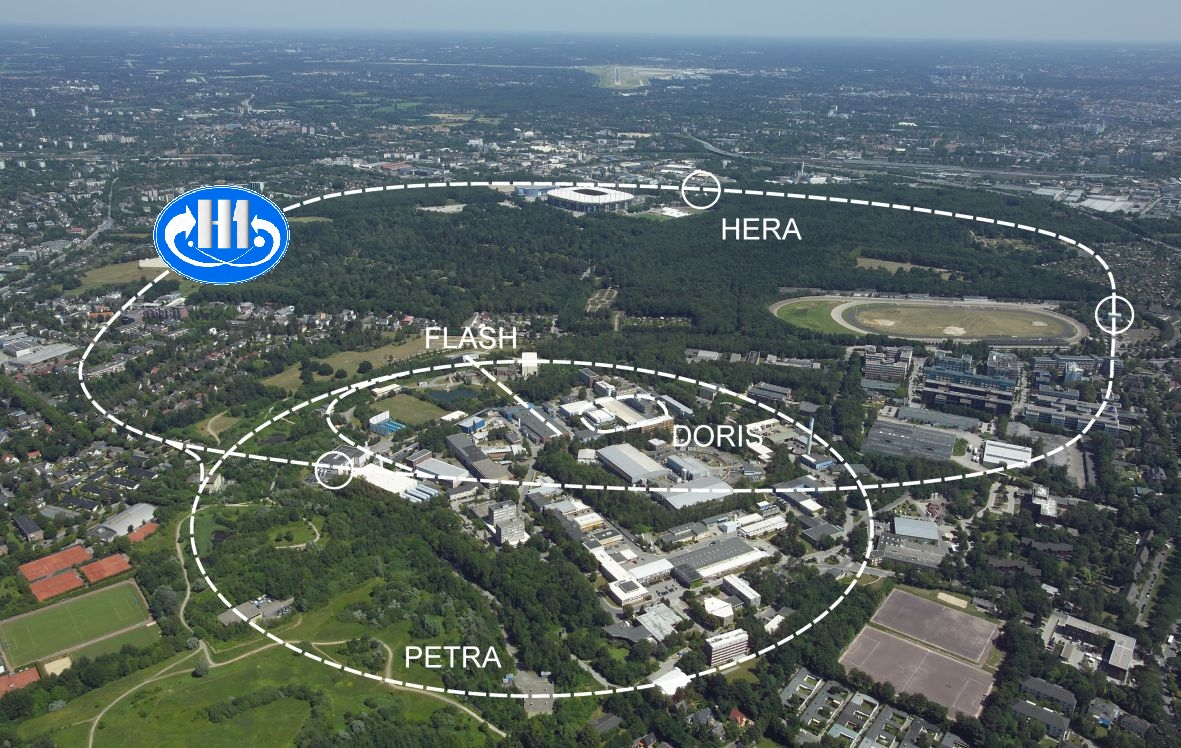
\includegraphics[width=0.7\textwidth]{images/DESY.jpg}
  \end{figure}
\end{frame}

\begin{frame}
  \begin{columns}
    \begin{column}{0.4\textwidth}
      Zahlen und Fakten zum HERA-Beschleuniger:
      \begin{itemize}
        \item{befindet sich am DESY in Hamburg, Deutschland}
        \item{Elektron-Proton-Speicherring}
        \item{Umfang: $6336 \,\mathrm{m}$}
        \item{lief von 1992 bis 2007}
        \item{Experimente: H1, ZEUS, Hermes}
        \item{Elektronen($30 \,\mathrm{GeV}$) und Protonen($820 \,\mathrm{GeV}$) treffen aufeinander}
        \item{Schwerpunktsenergie: $\sqrt{s} = 320 \,\mathrm{GeV} $}
        \item{Datenauswertung: Bis heute}
      \end{itemize}
    \end{column}

    \begin{column}{0.6\textwidth}
      \begin{figure}
        \centering
        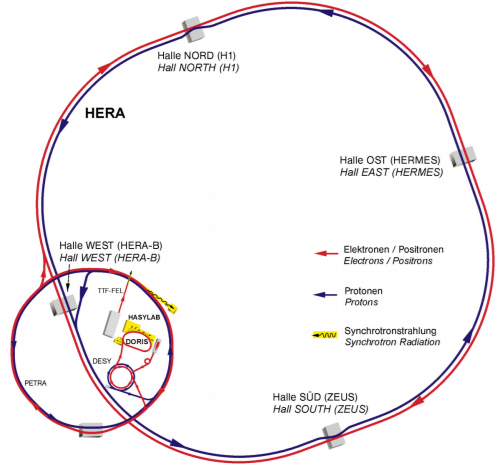
\includegraphics[width=0.6\textwidth]{images/hera.png}
      \end{figure}
      \centering
      \begin{itemize}
        \item{ \textcolor{red}{Rot:} Elektronen }
        \item{ \textcolor{blue}{Blau:} Protonen }
      \end{itemize}
    \end{column}
 \end{columns}
\end{frame}

\subsection{Der ZEUS-Detekror}
\begin{frame}{Der ZEUS-Detektor}
Eckdaten:
  \begin{itemize}
    \item{befindet sich in der Süd-Halle von HERA}
    \item{Maße: $12 \,\mathrm{m} \times 10 \,\mathrm{m} \times 19 \,\mathrm{m}  $  } 
    \item{Gewicht: $3600 \,\mathrm{Tonnen}$ } 
    \item{Aufgabe: Entschlüsselung der Struktur des Protons}
  \end{itemize}
\end{frame}

\begin{frame}{Aufbau}
  \begin{columns}
    \begin{column}{0.4\textwidth}
      \begin{itemize}
        \item {Uran Szintillator Kalorimeter (CAL)}
        \begin{itemize}
          \item {Misst Energie und Richtung der Teilchen}
          \item {Es umschließt verschiedene  Spurdetektoren}
          %\item {Vertex-Detektor(VXD), Zentrale Drift Kammer (CTD), Vorwärts(FTD) und Rückwärts (RTD) Drift Kammern, sowie einen Übergangsstrahlungsdetektor (TRD) }
          \item{Energie, die nicht völlig absorbiert wurde, wird im Begleit-Kalorimeter absorbiert}
        \end{itemize}
          \item{Vetowand}
          \begin{itemize}
            \item {Detektiert Hintergrunds-Ereignisse}
          \end{itemize}
          \item {Proton-Kalorimeter}
          \item {Luminositätsmonitor}
          \begin{itemize}
            \item {Detektiert Elektronen und Photonen aus Elektronenstrahlen}
          \end{itemize}
          \item{Solenoid ($1.8 \,\mathrm{T} $)}
      \end{itemize}
    \end{column}

    \begin{column}{0.6\textwidth}
      \begin{figure}
        \centering
        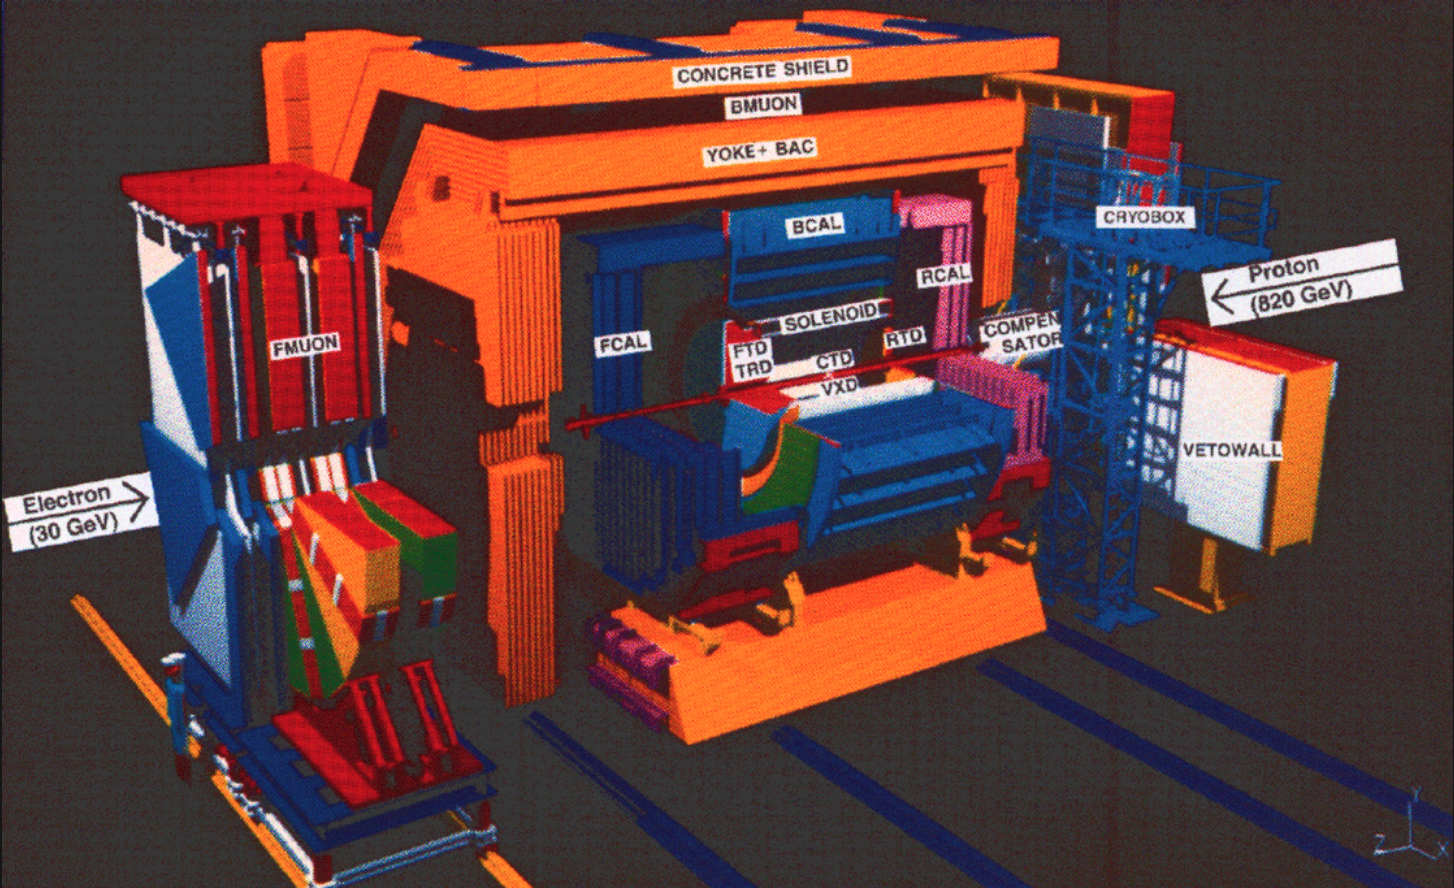
\includegraphics[width=0.8\textwidth]{images/Zeus.png}
      \end{figure}
    \end{column}
  \end{columns}
\end{frame}

\begin{frame}
  \begin{figure}
    \centering
    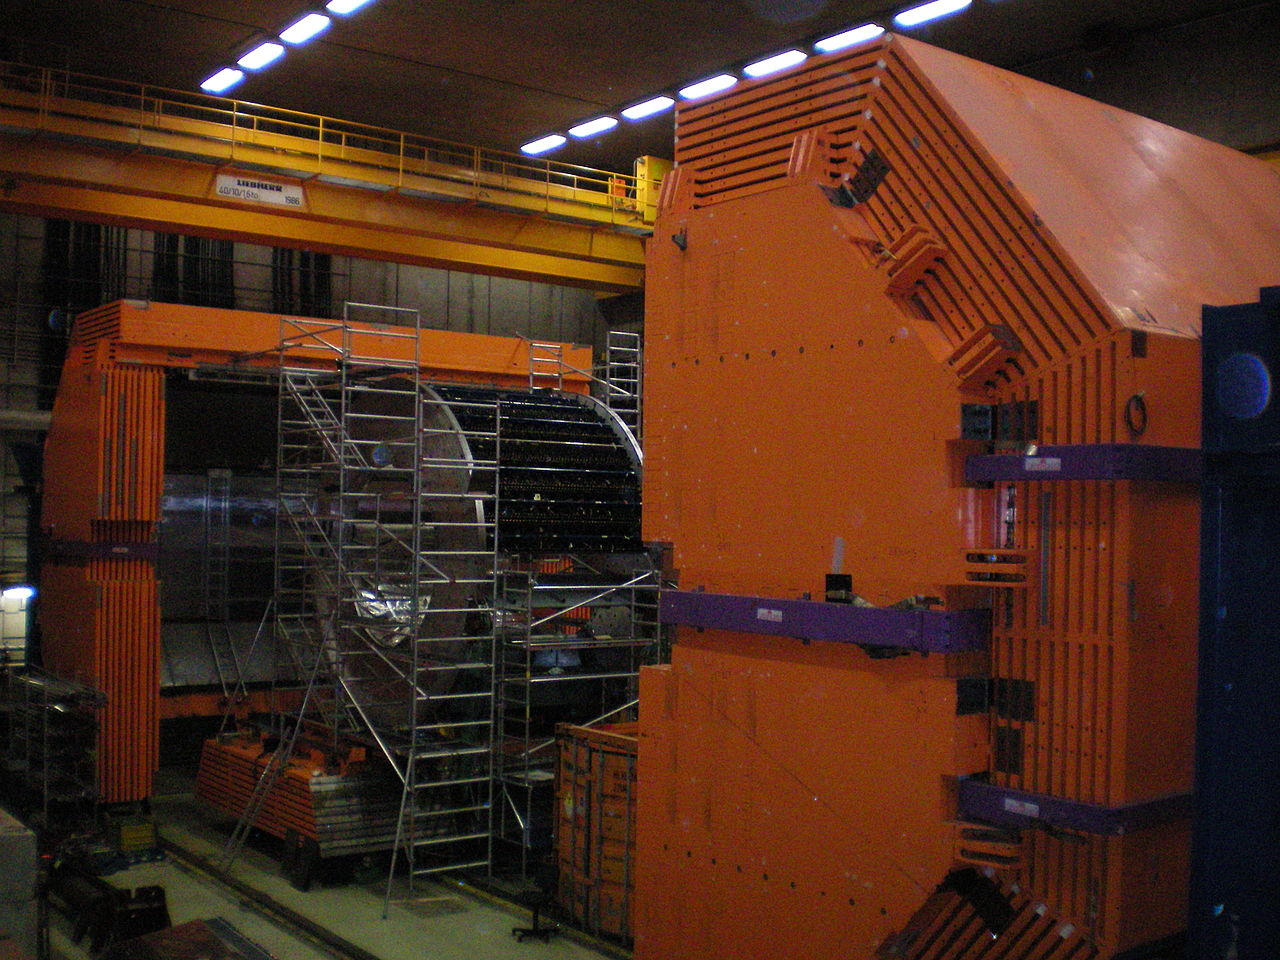
\includegraphics[width=0.6\textwidth]{images/Zeus-Real.jpeg}
  \end{figure}
\end{frame}

\subsection{Der H1-Detektor}

\begin{frame}{Der H1-Detektor}
  Eckdaten:
  \begin{itemize}
    \item{befindet sich in der Nord-Halle von HERA}
    \item{Maße: $12 \,\mathrm{m} \times 10 \,\mathrm{m} \times 15 \,\mathrm{m}  $  } 
    \item{Gewicht: $2800 \,\mathrm{Tonnen}$ } 
    \item{Aufgabe: Entschlüsselung der Struktur des Protons}
  \end{itemize}
\end{frame}

\begin{frame}{Aufbau}
  \begin{columns}
    \begin{column}{0.4\textwidth}
      \begin{itemize}
        \item{Asymmetrischer Aufbau}
        \item{Aufbau besteht aus:}
        \begin{itemize}
          \item{Spurenkammer}
          \item{Hadronisches Kalorimeter}
          \item{Elektromagnetisches Kalorimeter}
          \item{Supraleitende Spule ($1,2\,\mathrm{T} $)}
          \item{Myon-Kammer}
        \end{itemize}
      \end{itemize}
    \end{column}

    \begin{column}{0.6\textwidth}
      \begin{figure}
        \centering
        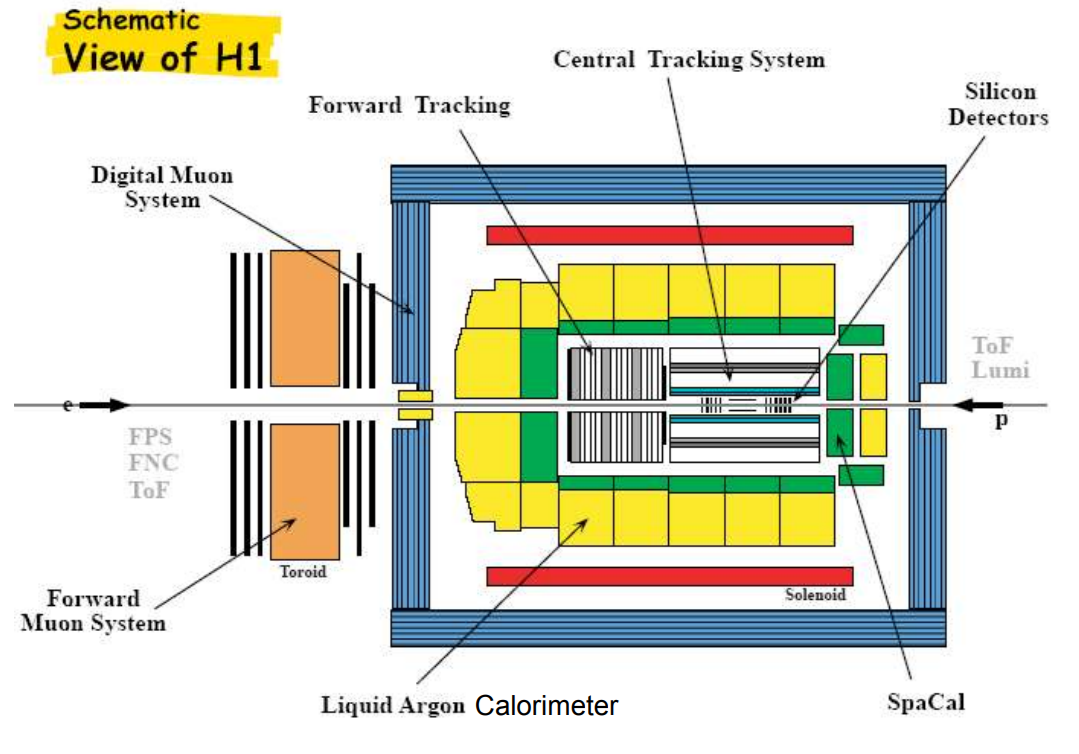
\includegraphics[width=0.9\textwidth]{images/H1.png}
      \end{figure}
    \end{column}
  \end{columns}
\end{frame}

\begin{frame}{Beispiel}
  ep $\rightarrow$ $\nu$ X
  \begin{figure}
    \centering
    \includegraphics[width=0.50\textwidth]{images/ep-vx.png}
  \end{figure}
\end{frame}

\begin{frame}
  \begin{figure}
    \centering
    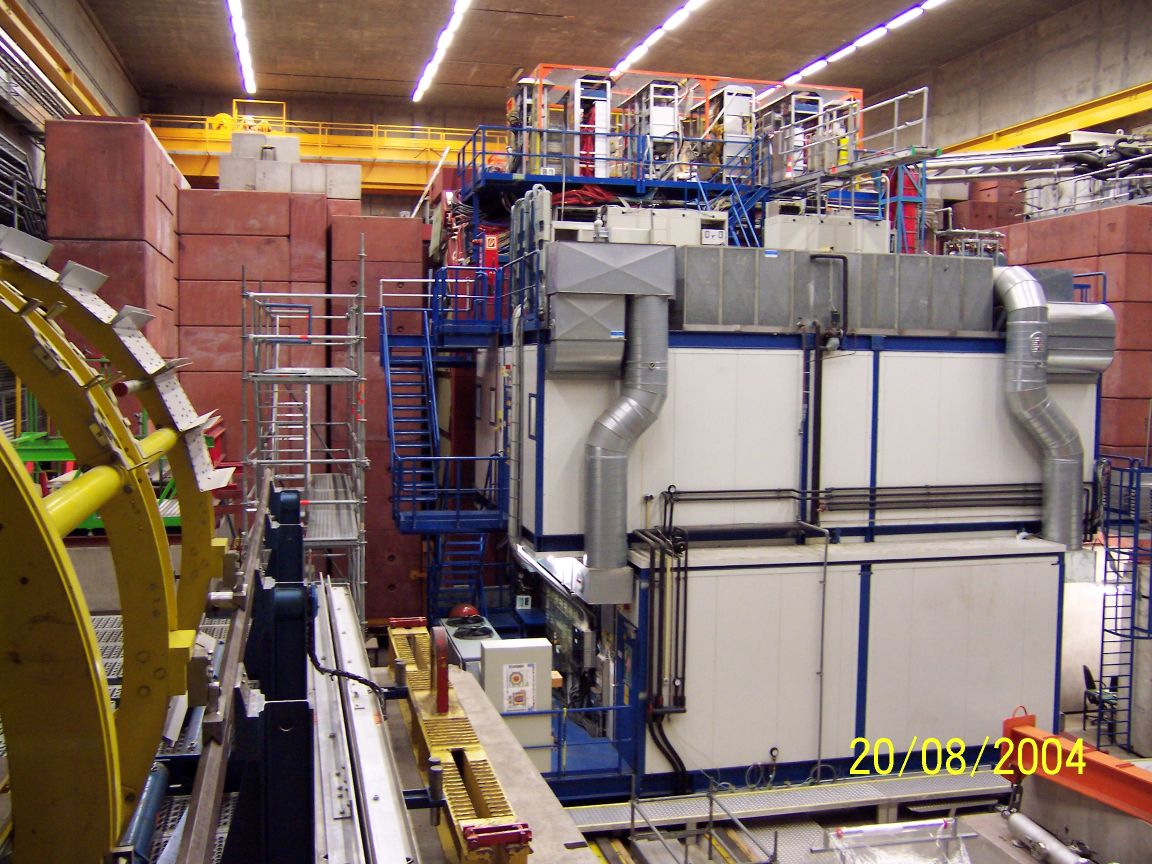
\includegraphics[width=0.65\textwidth]{images/H1_detector.jpg}
  \end{figure}
\end{frame}


\section{Ergebnisse}

\begin{frame}{Skalenbrechung}
  \begin{columns}
    \begin{column}{0.3\textwidth}
      \begin{itemize}
        \item{Größeres $Q^2$: mehr Quarks mit kleinem Bjorken-$x$}
        \begin{itemize}
          \item{mehr Quarks mit kleinem Bjorken-$x$}
          \item{weniger Quarks mit großem Bjorken-$x$}
        \end{itemize}
      \end{itemize}
    \end{column}

    \begin{column}{0.7\textwidth}
      \begin{figure}
        \centering
        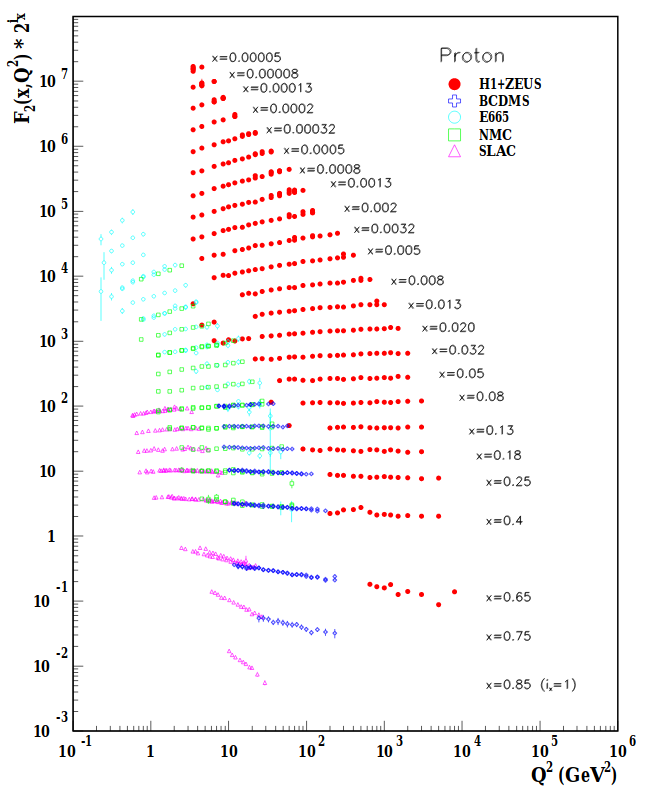
\includegraphics[width=0.55\textwidth]{images/Skalen.png}
      \end{figure}
    \end{column}
  \end{columns}
\end{frame}


\begin{frame}{Proton PDF}
  \begin{columns}
    \begin{column}{0.55\textwidth}
      \begin{figure}
    \centering
    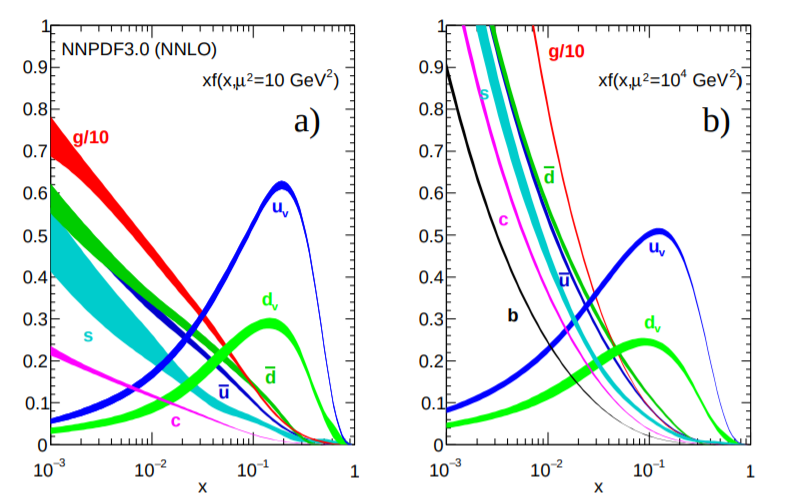
\includegraphics[scale=0.30]{images/Proton-PDF.png}
  \end{figure}
    \end{column}

    \begin{column}{0.45\textwidth}
      \begin{itemize}
        %\item{Messung veröffentlicht im Particle Data Group, Chin. Phys. C 40 (2016) 100001}
        \item{Das Proton besteht nicht nur Valenzquarks, es sind auch See-Quarks und Gluonen zu finden}
        \item{Es lässt sich beobachten:}
        \begin{itemize}
          \item { $\displaystyle \int_{0}^1 u_\text{v} \symup{d}x = 2$ und  $\displaystyle  \int_{0}^1 d_\text{v} \symup{d}x = 1$ }
          \item { $\displaystyle  \int_{0}^1 x \left[ u(x)+\bar{u}(x) + d(x)+\bar{d}(x) + s(x)+\bar{s}(x) \right] \symup{d}x = 1 - \frac{p_\text{g}}{p}$ beobachten }
        \end{itemize}
        \item{Struktur doch nicht unabhängig von $Q^2$.}
        \item{Größeres $Q^2 \rightarrow $ mehr Quarks mit kleinem $x$}
      \end{itemize}
    \end{column}

  \end{columns}
\end{frame}

\section{Weitere Experimente}
\begin{frame}{Weitere Experimente und was sie abdecken}
  \begin{figure}
    \centering
    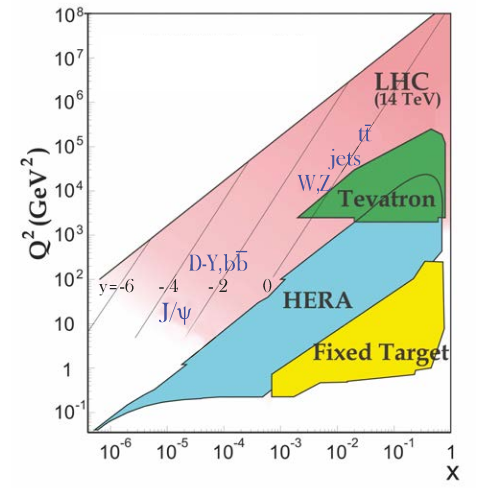
\includegraphics[scale=0.35]{images/Experimente.png}
  \end{figure}
\end{frame}

\section{Zusammenfassung}
\begin{frame}{Zusammenfassung}
  \begin{columns}
    \begin{column}{0.4\textwidth}
      \begin{itemize}
        \item{H1 und ZEUS liefern hohe Präzission über den Inhalt des Protons}
        \item{Proton besteht nicht nur aus den 3 Valenzquarks}
        \begin{itemize}
          \item{es besteht ebenfalls aus See-Quarks}
          \item{und Gluonen}
        \end{itemize}
        \item{Struktur ist abhängig von $Q^2$}
        \item{Wissen über Proton Struktur wichtig für weitere Experimente wie LHC}
      \end{itemize}
    \end{column}

    \begin{column}{0.6\textwidth}
      \begin{figure}
        \centering
        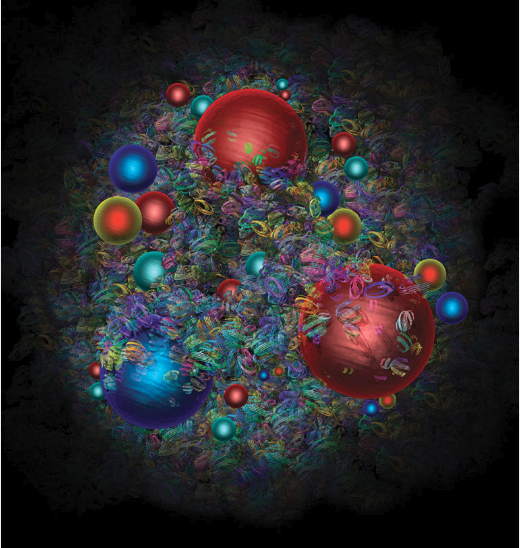
\includegraphics[width=0.7\textwidth]{images/proton-courier.png}
      \end{figure}
    \end{column}
  \end{columns}
\end{frame}

\begin{frame}
\centering
\Huge{Vielen Dank für Eure Aufmerksamkeit!}
\end{frame}

\end{document}